\documentclass[11pt,openany]{article}

\usepackage{mathtools, commath}
% Packages for formatting
\usepackage[margin=1in]{geometry}
\usepackage{fancyhdr}
\usepackage{enumerate}
\usepackage{graphicx}
\usepackage{kotex}
\usepackage{arydshln} % Include this package
\usepackage{bbding}
\usepackage{amsmath}
\usepackage{amsthm}
\usepackage[dvipsnames,table]{xcolor}
\usepackage{amssymb, amsfonts}
\usepackage{wasysym}
\usepackage{footnote}
\usepackage{tablefootnote}
\usepackage{arydshln} % Include this package
% Fonts
\usepackage[T1]{fontenc}
\usepackage[utf8]{inputenc}
\usepackage{newpxtext,newpxmath}
\usepackage{sectsty}

% Define colors
\definecolor{TealBlue1}{HTML}{0077c2}
\definecolor{TealBlue2}{HTML}{00a5e6}
\definecolor{TealBlue3}{HTML}{b3e0ff}
\definecolor{TealBlue4}{HTML}{00293c}
\definecolor{TealBlue5}{HTML}{e6f7ff}

\definecolor{thmcolor}{RGB}{231, 76, 60}
\definecolor{defcolor}{RGB}{52, 152, 219}
\definecolor{lemcolor}{RGB}{155, 89, 182}
\definecolor{corcolor}{RGB}{46, 204, 113}
\definecolor{procolor}{RGB}{241, 196, 15}

\usepackage{color,soul}
\usepackage{soul}
\newcommand{\mathcolorbox}[2]{\colorbox{#1}{$\displaystyle #2$}}
\usepackage{cancel}
\newcommand\crossout[3][black]{\renewcommand\CancelColor{\color{#1}}\cancelto{#2}{#3}}
\newcommand\ncrossout[2][black]{\renewcommand\CancelColor{\color{#1}}\cancel{#2}}

\usepackage{hyperref}
\usepackage{booktabs}

% Chapter formatting
\definecolor{titleTealBlue}{RGB}{0,53,128}
\usepackage{titlesec}
\titleformat{\section}
{\normalfont\sffamily\Large\bfseries\color{titleTealBlue!100!gray}}{\thesection}{1em}{}
\titleformat{\subsection}
{\normalfont\sffamily\large\bfseries\color{titleTealBlue!50!gray}}{\thesubsection}{1em}{}

%Tcolorbox
\usepackage[most]{tcolorbox}
\usepackage{multirow}
\usepackage{multicol}

\usepackage[linesnumbered,ruled]{algorithm2e}
\usepackage{algpseudocode}
\usepackage{setspace}
\SetKwComment{Comment}{/* }{ */}
\SetKwProg{Fn}{Function}{:}{end}
\SetKw{End}{end}
\SetKw{DownTo}{downto}

% Define a new environment for algorithms without line numbers
\newenvironment{algorithm2}[1][]{
	% Save the current state of the algorithm counter
	\newcounter{tempCounter}
	\setcounter{tempCounter}{\value{algocf}}
	% redefine the algorithm numbering (remove prefix)
	\renewcommand{\thealgocf}{}
	\begin{algorithm}
	}{
	\end{algorithm}
	% Restore the algorithm counter state
	\setcounter{algocf}{\value{tempCounter}}
}

\usepackage{adjustbox}
% Header and footer formatting
\pagestyle{fancy}
\fancyhead{}
\fancyhf{}
\rhead{\textcolor{TealBlue2}{\large\textbf{기대수(기초부터 대학원 수학까지 시리즈) 3기}}}%\rule{3cm}{0.4pt}}
\lhead{\textcolor{TealBlue2}{\large\textbf{수학의 즐거움, Enjoying Math}}}
% Define footer
%\newcommand{\footer}[1]{
%\begin{flushright}
%	\vspace{2em}
%	\includegraphics[width=2.5cm]{school_logo.jpg} \\
%	\vspace{1em}
%	\textcolor{TealBlue2}{\small\textbf{#1}}
%\end{flushright}
%}
%\rfoot{\large Department of Information Security, Cryptogrphy and Mathematics, Kookmin Uni.\includegraphics[height=1.5cm]{school_logo.jpg}}
\fancyfoot{}
\fancyfoot[C]{-\thepage-}

\usepackage{tcolorbox}
\tcbset{colback=white, arc=5pt}

\definecolor{axiomcolor}{HTML}{a88bfa}
\definecolor{defcolor}{RGB}{52, 152, 219}
\definecolor{procolor}{RGB}{241, 196, 15}
\definecolor{thmcolor}{RGB}{231, 76, 60}
\definecolor{lemcolor}{RGB}{155, 89, 182}
\definecolor{corcolor}{RGB}{46, 204, 113}
\definecolor{execolor}{RGB}{90, 128, 127}

% Define a new command for the custom tcolorbox
\newcommand{\axiombox}[2][]{%
	\begin{tcolorbox}[colframe=axiomcolor, title={\color{white}\bfseries #1}]
		#2
	\end{tcolorbox}
}

\newcommand{\defbox}[2][]{%
	\begin{tcolorbox}[colframe=defcolor, title={\color{white}\bfseries #1}]
		#2
	\end{tcolorbox}
}

\newcommand{\lembox}[2][]{%
	\begin{tcolorbox}[colframe=lemcolor, title={\color{white}\bfseries #1}]
		#2
	\end{tcolorbox}
}

\newcommand{\probox}[2][]{%
	\begin{tcolorbox}[colframe=procolor, title={\color{white}\bfseries #1}]
		#2
	\end{tcolorbox}
}

\newcommand{\thmbox}[2][]{%
	\begin{tcolorbox}[colframe=thmcolor, title={\color{white}\bfseries #1}]
		#2
	\end{tcolorbox}
}

\newcommand{\corbox}[2][]{%
	\begin{tcolorbox}[colframe=corcolor, title={\color{white}\bfseries #1}]
		#2
	\end{tcolorbox}
}



\usepackage{amsthm}

% Define custom theorem styles
\newtheoremstyle{dotless} % Name of the style
{3pt} % Space above
{3pt} % Space below
{\itshape} % Body font
{} % Indent amount
{\bfseries} % Theorem head font
{} % Punctuation after theorem head
{2.5mm} % Space after theorem head
{} % Theorem head spec

\newtheoremstyle{definitionstyle} % Name of the style
{3pt} % Space above
{3pt} % Space below
{} % Body font
{} % Indent amount
{\bfseries} % Theorem head font
{.} % Punctuation after theorem head
{2.5mm} % Space after theorem head
{} % Theorem head spec

% Applying custom styles
\theoremstyle{dotless}
\newtheorem{theorem}{Theorem} % Theorem environment with section-wise numbering
\newtheorem{proposition}[theorem]{Proposition} % Theorem environment with section-wise numbering
\newtheorem{lemma}[theorem]{Lemma} % Lemma shares the counter with theorem
\newtheorem{corollary}[theorem]{Corollary} % Corollary shares the counter with theorem

\theoremstyle{definitionstyle}
\newtheorem*{observation}{\textcolor{Magenta}{Observation}}
\newtheorem{definition}{Definition} % Definition shares the counter with theorem
\newtheorem{example}{Example} % Example shares the counter with theorem
\newtheorem{exercise}{Exercise} % Example shares the counter with theorem
\newtheorem{remark}{Remark} % Remark shares the counter with theorem
\newtheorem*{note}{Note}

\newtheorem*{definition*}{Definition} % Definition shares the counter with theorem
\newtheorem*{example*}{Example} % Example shares the counter with theorem
\newtheorem*{exercise*}{\textcolor{violet}{Exercise}} % Example shares the counter with theorem
\newtheorem*{remark*}{Remark} % Remark shares the counter with theorem


\usepackage{tikz}
\usepackage{tikz-cd}
\usepackage{tikz-3dplot}
\usepackage{pgfplots}
\pgfplotsset{compat=newest} % Adjust to your version of pgfplots
\def\Circlearrowleft{\ensuremath{%
		\rotatebox[origin=c]{180}{$\circlearrowleft$}}}
\def\Circlearrowright{\ensuremath{%
		\rotatebox[origin=c]{180}{$\circlearrowright$}}}
\def\CircleArrowleft{\ensuremath{%
		\reflectbox{\rotatebox[origin=c]{180}{$\circlearrowleft$}}}}
\def\CircleArrowright{\ensuremath{%
		\reflectbox{\rotatebox[origin=c]{180}{$\circlearrowright$}}}}
\usetikzlibrary{
	3d, % For 3D drawing
	angles,
	arrows,
	arrows.meta,
	backgrounds,
	bending,
	calc,
	decorations.pathmorphing,
	decorations.pathreplacing,
	decorations.markings,
	fit,
	matrix,
	patterns,
	patterns.meta,
	positioning,
	quotes,
	shadows,
	shapes,
	shapes.geometric,
	tikzmark
}
\tikzset{
	% single mid‐path arrow
	mid arrow/.style={
		decoration={
			markings,
			mark=at position 0.5 with {\arrow{Stealth[scale=1.2]}}
		},
		postaction={decorate},
	},
	% style for field arrows
	field arrow/.style={
		-{Stealth[scale=1.0]},
		thick,
		blue!70!black,
	},
}
\newcommand{\ie}{\textnormal{i.e.}}
\newcommand{\rsa}{\mathsf{RSA}}
\newcommand{\rsacrt}{\mathsf{RSA}\textendash\mathsf{CRT}}
\newcommand{\inv}[1]{#1^{-1}}

%New Command
%\newcommand{\set}[1]{\left\{#1\right\}}
\newcommand{\N}{\mathbb{N}}
\newcommand{\Z}{\mathbb{Z}}
\newcommand{\Q}{\mathbb{Q}}
\newcommand{\R}{\mathbb{R}}
\newcommand{\cR}{\mathcal{R}}
\newcommand{\C}{\mathbb{C}}
\newcommand{\F}{\mathbb{F}}
\newcommand{\nbhd}{\mathcal{N}}
\newcommand{\Log}{\operatorname{Log}}
\newcommand{\Arg}{\operatorname{Arg}}
\newcommand{\pv}{\operatorname{P.V.}}

\newcommand{\of}[1]{\left( #1 \right)} 
%\newcommand{\abs}[1]{\left\lvert #1 \right\rvert}
%\newcommand{\norm}[1]{\left\| #1 \right\|}

\newcommand{\sol}{\textcolor{magenta}{\bf Sol}}
\newcommand{\conjugate}[1]{\overline{#1}}

\newcommand{\res}{\operatorname{res}}
\DeclareMathOperator*{\Res}{\operatorname{Res}}

%\renewcommand{\Re}{\operatorname{Re}}
%\renewcommand{\Im}{\operatorname{Im}}

\newcommand{\cyclic}[1]{\langle #1 \rangle}
\newcommand{\uniform}{\overset{\$}{\leftarrow}}
\newcommand{\xmark}{\textcolor{red}{\XSolidBrush}}
\newcommand{\vmark}{\textcolor{green!75!black}{\CheckmarkBold}}

\newcommand{\gen}[1]{\langle #1 \rangle}
\newcommand{\Gen}[1]{\left\langle #1 \right\rangle}

\newcommand{\img}[1]{\text{Img}(#1)}
\newcommand{\Img}[1]{\text{Img}\left(#1\right)}
\newcommand{\preimg}[1]{\text{Img}^{-1}(#1)}
\newcommand{\Preimg}[1]{\text{Img}^{-1}\left(#1\right)}

\newcommand{\relation}{\mathrel{\mathcal{R}}}
\newcommand{\injection}{\rightarrowtail}
\newcommand{\surjection}{\twoheadrightarrow}
\newcommand{\id}{\textnormal{id}}

\newcommand{\eqclass}[1]{\left[#1\right]}

% Define custom colors for O and X
\newcommand{\yes}{\textcolor{blue}{\bf \fullmoon}}
\newcommand{\no}{\textcolor{red}{\bf \texttimes}}

\DeclarePairedDelimiter\ceil{\lceil}{\rceil}
\DeclarePairedDelimiter\floor{\lfloor}{\rfloor}
%\renewcommand{\floor}[#1]{\lfloor #1\rfloor}
%\newcommand{\Floor}[#1]{\left\lfloor #1\right\rfloor}
%\newcommand{\ceil}[#1]{\lceil #1\rceil}
%\newcommand{\Ceil}[#1]{\left\lceil #1\right\rceil}

\newcommand{\topology}{\mathscr{T}}
\newcommand{\sequence}[1]{\langle #1\rangle}

\setstretch{1.25}
\begin{document}
\pagenumbering{arabic}
\begin{center}
	\huge\textbf{Advanced Calculus III}\\
	\vspace{0.5em}
	\large{Ji, Yong-hyeon}\\
%	\large{\ttfamily \url{https://github.com/Hacker-Code-J}}\\
	\vspace{0.5em}
	\normalsize{\today}\\
\end{center}

\noindent 
We cover the following topics in this note.
\begin{itemize}
	\item Limit of a Function
	\item Continuity of a Function
	\item TBA
\end{itemize}
\hrule\vspace{12pt}
\defbox[Limit Point (Metric Space)]{\begin{definition*}
	Let $(X,d)$ be a metric space. Let $S\subseteq X$ and $\alpha\in X$. A point $p\in X$ is a \textbf{limit point} of $S$ if and only if 
	\[
	\forall\varepsilon>0,\ B_{\varepsilon}(\alpha)\cap (S\setminus\set{p})\neq\varnothing.
	\] That is, \[
	\forall\varepsilon>0,\ \set{x\in S:0< d(x,p)<\varepsilon}\neq\varnothing.
	\]
\end{definition*}}
\begin{remark}
	Note that $\alpha$ does not have to be an element of $A$ to be a limit point.
\end{remark}

\newpage
\begin{note}[Limit Point (Topology)]
	Let $(X,\tau)$ be a topological space. For a subset $S\subseteq X$. A point $p\in X$ is a limit point of $S$ if and only if \[
	\forall U\in\tau\ \text{with}\ p\in U,\ U\cap (S\setminus\set{p})\neq\varnothing.
	\]
\end{note}
\begin{example}
\begin{tikzpicture}[scale=2]
	
	% Draw the x-axis
	\draw[->] (-0.5, 0) -- (4.5, 0) node[right] {$n$ (Index)};
	% Draw the y-axis
	\draw[->] (0, -0.5) -- (0, 2.5) node[above] {$a_n$ (Value)};
	
	% Draw the limit point
	\draw[dashed, red] (-0.5, 2) -- (4.5, 2) node[right] {Limit $L$};
	\filldraw[red] (0, 2) circle (1.5pt);
	
	% Label for limit point
	\node[red, right] at (0, 2.1) {Limit $L = 2$};
	
	% Plot points for the sequence
	\foreach \n/\y in {1/1.5, 2/1.8, 3/1.9, 4/1.95} {
		\filldraw[blue] (\n, \y) circle (1.5pt);
	}
	
	% Sequence points labels
	\node[blue, above] at (1, 1.5) {$a_1$};
	\node[blue, above] at (2, 1.8) {$a_2$};
	\node[blue, above] at (3, 1.9) {$a_3$};
	\node[blue, above] at (4, 1.95) {$a_4$};
	
	% Label for sequence behavior
	\node[blue] at (2, 0.3) {Sequence: $a_n = 2 - \frac{1}{n}$};
	
\end{tikzpicture}
\end{example}
%\begin{center}
%\begin{tikzpicture}[scale=3]
%	% Draw the coordinate axes
%%	\draw[->] (-2, 0) -- (4, 0) node[right] {x};
%%	\draw[->] (0, -2) -- (0, 4) node[above] {y};
%	% Define the set of points
%	\foreach \x/\y in {0.5/1, 1.5/0.5, 2/1.5, 2.5/2.2, 1.8/2.5, 1.2/2.3, 0.8/1.8} {
%		\fill[blue] (\x, \y) circle[radius=2pt];
%	}
%	% Highlight the limit point
%	\fill[red] (2, 1) circle[radius=2.5pt] node[below right] {$\alpha$};
%	% Draw the open ball
%	\draw[green!60!black, thick, dashed] (2, 1) circle (1);
%	\node[green!60!black] at (3, 2) {$B_\varepsilon(\alpha)$};
%	% Annotate nearby points in the open ball
%	\foreach \x/\y in {1.5/0.5, 2/1.5, 2.5/2.2} {
%		\draw[->, orange, thick] (\x, \y) -- (2, 1);
%	}
%	
%	% Explanation of other points
%	\node[blue] at (0.5, 0.5) {Other points in the set};
%	\node[red] at (2.8, 0.8) {Limit point $p$};
%\end{tikzpicture}
%\end{center}
\defbox[$\star$ Limit of a Function ($\epsilon-\delta$) $\star$]{\begin{definition*}
	Let $f:X\to\R$ be a function defined on a subset $X\subseteq\R$ of a topological space, and let $p\in X$ be a limit point of $X$. We say that $L\in\R$ is the \textbf{limit of the function $f$ as $x$ approaches $p$} if
	\[
	\boxed{\forall\varepsilon>0,\ \exists\delta>0\ \text{such that}\ \forall x\in X,\ 0<\abs[0]{x-p}<\delta\implies\abs[0]{f(x)-L}<\varepsilon}.
	\] We write \[
	\boxed{\lim\limits_{x\to p} f(x)=L}.
	\]
\end{definition*}}
\begin{center}
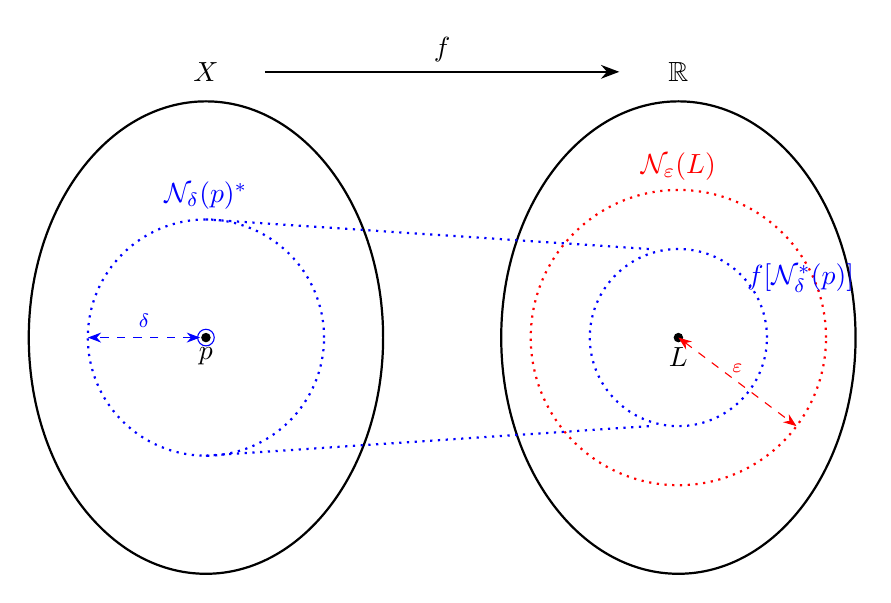
\begin{tikzpicture}[scale=1.5]
	\draw[thick] (-2,0) ellipse (1.5 and 2);
	\draw[blue, dotted, thick] (-2,0) ellipse (1 and 1);
	\node[above, blue] at (-2,1) {$\nbhd_\delta(p)^*$};
	\draw[thick] (2,0) ellipse (1.5 and 2);
	\node[red, above] at (2,1.25) {$\nbhd_\varepsilon(L)$};
	\draw[red, dotted, thick] (2,0) ellipse (1.25 and 1.25);
	\draw[blue, dotted, thick] (2,0) ellipse (.75 and .75);
	\node[blue, right, align=left] at (2.5,.5) {$f[\nbhd_\delta^* (p)]$};
	
	% Labels for sets
	\node at (-2, 2.25) {$X$};
	\node at (2, 2.25) {$\R$};
	
	% Draw the arrows representing the function
	\draw[-Stealth, thick] (-1.5, 2.25) -- (1.5,2.25) node[midway, above] {$f$};
	
	%	\node at (2, 1.25) {$f[A]$};
	\draw[blue, dotted, thick] (-2, 1) -- (1.75, .75);
	\draw[blue, dotted, thick] (-2, -1) -- (1.75, -.75);
	
	\filldraw (-2,0) circle (1pt) node[below] {$p$};
	\draw[blue] (-2,0) circle (2pt);
	\filldraw (2,0) circle (1pt) node[below] {$L$};
%	\draw[|->] (-1.85, 0) -- (1.85, 0);
	
	\draw[>=Stealth, <->, dashed, red] (2, 0) -- (3,-.75) node[midway, above] {\scriptsize $\varepsilon$};
	\draw[>=Stealth, <->, dashed, blue] (-2.05, 0) -- (-3,0) node[midway, above] {\scriptsize $\delta$};
\end{tikzpicture}
\end{center}
\begin{remark}
\[
\lim\limits_{x\to p} f(x)\neq L\iff \exists\varepsilon>0:[\forall\delta>0:\exists x\in X: 0<\abs[0]{x-p}<\delta\ \text{but}\ \abs[0]{f(x)-L}>0].
\]
\end{remark}

\defbox[Continuity of a Function]{\begin{definition*}
	Let $f:X\to\R$ be a function defined on a subset $X\subseteq\R$ of a topological space, and let $p\in X$. The function $f$ is said to be $f$ is \textbf{continuous at $p$} if and only if \[
	\lim\limits_{x\to p}f(x)=f(p).
	\] That is, \[
	\forall\varepsilon>0,\ \exists\delta>0\ \text{such that}\ \abs{x-p}<\delta\implies|f(x)-f(p)|<\varepsilon.
	\]
\end{definition*}}
\begin{remark}[Continuity of a Set]
	The function $f$ is continuous on subset $S\subseteq X$ if it it continuous at every point $p\in S$.
\end{remark}
\begin{remark}[Continuity in a Topological Space]
	Let $(X,\tau_X)$ and $(Y,\tau_Y)$ are topological spaces. $f:X\to Y$ is \textbf{continuous} if and only if $$U_Y\in\tau_Y\implies f^{-1}[U_Y]\in\tau_X,$$ where $f^{-1}[U_Y]=\set{x\in X:f(x)\in U_Y}$ is the preimage of $U_Y$ under $f$.
\end{remark}

\newpage
%\begin{note}[Subsequence]
%	Let $\set{a_n}$ be a sequence of real numbers, and let $n_1<n_2<\cdots<n_k<\cdots$ be a strictly increasing of natural numbers. Then $\set{a_{n_k}}$ is called \textbf{subsequence} of $\set{a_n}$.
%\end{note}
\begin{note}
	$[p\Rightarrow(q\Rightarrow r)]\equiv [p\Rightarrow(\lnot q\lor r)]\equiv[\lnot p\lor (\lnot q\lor r)]\equiv [\lnot (p\land q)\lor r]\equiv [(p\land q)\Rightarrow r]$.
\end{note}
\thmbox[Limit of Function by Convergent Sequences]{\begin{theorem*}
Let $f:X\to\R$ be a function defined on a subset $\varnothing\neq X\subseteq\R$ of a topological space, and let $p$ is a limit point of $X$. Then \[
\lim\limits_{x\to p}f(x)=L\iff\left[\forall\set{x_n}\subseteq X\setminus\set{p},\left(\lim\limits_{n\to\infty}x_n=p\implies\lim\limits_{n\to\infty}f(x_n)=L\right)\right].
\]
\end{theorem*}}
\begin{proof}
\begin{itemize}
	\item[($\Rightarrow$)] Suppose that $\lim\limits_{x\to p}f(x)=L$. Let $\set{x_n}\subseteq X\setminus\set{p}$ be a sequence, and let $\lim\limits_{n\to\infty}x_n=p$. We NTS that \[
	\lim\limits_{n\to\infty}f(x_n)=L,\quad\ie,\color{blue}\quad\forall\varepsilon>0:\exists N\in\N:n\geq N\Rightarrow\abs[0]{f(x_n)-L}<\varepsilon.
	\] \textcolor{blue}{Let $\varepsilon>0$}. Since $\lim\limits_{x\to p}f(x)=L$, we know \begin{equation*}
		\exists\delta>0\ \text{such that}\ 0<\abs[0]{x-p}<\delta\implies\abs[0]{f(x)-L}<\varepsilon.\tag{*}
	\end{equation*} Since $\lim\limits_{n\to\infty}x_n=p$, we obtain \[
	\textcolor{blue}{\exists N\in\N}\ \text{such that}\ n\geq N\implies\abs[0]{x_n-p}<\delta.
	\] Thus, \textcolor{blue}{if $n\geq N$ then}, \begin{align*}
		\abs[0]{x_n-p}<\delta&\implies 0<\abs[0]{x_n-p}<\delta\quad\because x_n\neq p \\
		&\implies\textcolor{blue}{\abs[0]{f(x_n)-L}<\varepsilon}\quad\text{by (*)}
	\end{align*} Thus, $\lim\limits_{n\to\infty}f(x_n)=L$.
	\item[($\Leftarrow$)] Let the RHS holds. Assume, for the contradiction, that $\lim\limits_{x\to p} f(x)\neq L$, \ie, \[
	\textcolor{green!50!black}{\exists\varepsilon>0}:\forall\delta>0:\exists x_\delta\in X:0<\abs[0]{x_\delta-p}<\delta\ \text{but}\ \textcolor{magenta}{\abs[0]{f(x_\delta)-L}\geq\varepsilon}.
	\] Take $\delta=1/n$. Then \[
	\exists x_n\in X\ \text{such that}\ 0<\abs[0]{x_n-p}<\delta\ \text{but}\ \abs[0]{f(x_n)-L}\geq \varepsilon.
	\] \textcolor{gray!50}{\st{(Axiom of Countable Choice)}}\ This means that \[
	\forall n\in\N:\exists\set{x_n}\subseteq X\setminus\set{p}\ \text{such that}\ 0<\abs[0]{x_n-p}<\frac{1}{n}\ \text{but}\ \textcolor{magenta}{\abs[0]{f(x_n)-L}\geq \varepsilon}.
	\] By Squeeze Theorem, we have $\lim\limits_{n\to\infty}x_n=p$ since $0<\abs[0]{x_n-p}<1/n$. Since the RHS holds, we know $\lim\limits_{n\to\infty}f(x_n)=L$. Then, for some $\textcolor{green!50!black}{\varepsilon>0}$, \[
	\exists N\in\N\ \text{such that}\ n\geq N\implies\textcolor{magenta}{\abs{f(x_n)-L}<\varepsilon}\ \text{\Large\lightning}.
	\]
\end{itemize}
\end{proof}
\corbox[Continuity of Function by Convergent Sequences]{\begin{corollary*}
Let $f:X\to\R$ be a function defined on a subset $\varnothing\neq X\subseteq\R$ of a topological space, and let $p$ is a limit point of $X$. Then \[
\lim\limits_{x\to p}f(x)=f(p)\iff\left[\forall\set{x_n}\subseteq X,\left(\lim\limits_{n\to\infty}x_n=p\implies\lim\limits_{n\to\infty}f(x_n)=f(p)\right)\right].
\]
\end{corollary*}}
\begin{proof}
	
\end{proof}

\thmbox[Sandwitch Theorem; Squeeze Theorem]{\begin{theorem*}
	
\end{theorem*}}
\begin{proof}
	content...
\end{proof}

\newpage
\thmbox[Monotone Convergence Theorem (MCT)]{\begin{theorem*}
	TBA
\end{theorem*}}
\begin{proof}
	TBA
\end{proof}

\thmbox[Nested Interval Property (NIP)]{\begin{theorem*}
	TBA
\end{theorem*}}
\begin{proof}
	TBA
\end{proof}

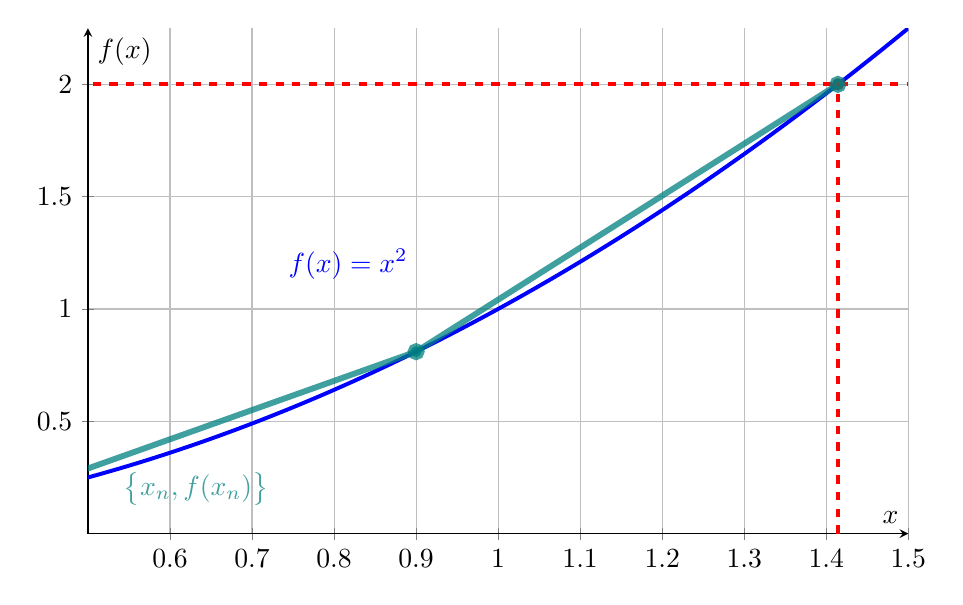
\begin{tikzpicture}
	
	% Create a pgfplots environment
	\begin{axis}[
		axis lines=middle,
		xlabel={$x$},
		ylabel={$f(x)$},
		xmin=.5, xmax=1.5,
		ymin=0, ymax=2.25,
		width=12cm,
		height=8cm,
		grid=both,
		legend style={font=\small},
		legend pos=north west,
		samples=100,
		domain=.5:1.5
		]
		
		% Continuous function f(x)
		\addplot[line width=.5mm, blue, domain=.5:1.5] {x^2} 
		node[pos=0.8, midway, left=2cm] {\textcolor{blue}{$f(x) = x^2$}};
		
		% Horizontal dashed line for limit L
		\addplot[red, dashed, line width=.5mm] coordinates {(0,2) (1.5,2)} 
		node[pos=0.9, above] {\textcolor{red}{}};
		\addplot[red, dashed, line width=.5mm] coordinates {({sqrt(2)},0) ({sqrt(2)},2)};
		
		% Point p (limit point)
		\addplot[mark=*, mark options={red}, only marks] coordinates {({sqrt(2)},2)} 
		node[below] {\textcolor{red}{}};
		
		% Sequence points approaching p
		\addplot[line width = .75mm, mark=*, teal, opacity=0.75] coordinates {(.4,{.4^2}) (.9,{.9^2}) ({sqrt(2)},2)}
		node[pos=0.1, below right] {\textcolor{teal}{$\set{x_n,f(x_n)}$}};
%		
%		% Annotate sequence x_n -> p
%		\draw[->, thick, orange] (axis cs:0.8,0) -- (axis cs:1,0) 
%		node[midway, below] {\textcolor{orange}{$x_n \to p$}};
%		
%		% Annotate f(x_n) -> L
%		\draw[->, thick, orange] (axis cs:0.99,0.9801) -- (axis cs:1,1) 
%		node[midway, right] {\textcolor{orange}{$f(x_n) \to L$}};
%		
%		% Neighborhood of p
%		\draw[<->, thick, red] (axis cs:0.85,-0.1) -- (axis cs:1.15,-0.1)
%		node[midway, below] {\textcolor{red}{$\delta$}};
		
		% Legend
%		\legend{
%			$f(x)$ (continuous),
%			Limit $L$,
%			Limit point $p$,
%			Sequence points $\{x_n\}$
%		}
		
	\end{axis}
	
\end{tikzpicture}


\vfill

\begin{thebibliography}{9}
	\bibitem{advanced_calc_e}
	수학의 즐거움, Enjoying Math. ``수학 공부, 기초부터 대학원 수학까지, 10. 해석학 개론 (e) 엡실론-델타와 수열의 수렴성'' YouTube Video, 25:57. Published 
	September 29, 2019. URL: \url{https://youtu.be/2Ml3G_Duffk?si=qo-CVgW3Ukd4ADRL}.
%	\bibitem{advanced_calc_f}
%	수학의 즐거움, Enjoying Math. ``수학 공부, 기초부터 대학원 수학까지, 11. 해석학 개론 (f) MCT and NIP'' YouTube Video, 20:17. Published 
%	October 1, 2019. URL: \url{https://youtu.be/YdnBQaY5eDk?si=BNe0Ue4iq2P9Fxsd}.
%	\bibitem{advanced_calc_g}
%	수학의 즐거움, Enjoying Math. ``수학 공부, 기초부터 대학원 수학까지, 12. 해석학 개론 (g) Limsup, Liminf'' YouTube Video, 34:31. Published 
%	October 2, 2019. URL: \url{https://youtu.be/4Q1cm3VQPUE?si=phAhKwnOxdnRAiRR}.
\end{thebibliography}
%\newpage
%\appendix
%\section{Complement of Family}
%\begin{note}
%	\[
%	\left(\bigcup_{i\in\Lambda}E_i\right)^C=
%	\bigcap_{i\in\Lambda}\left(E_i\right)^C
%	\]
%	\begin{proof}
%		content...
%	\end{proof}
%\end{note}
\end{document}
